\chapter{Środowisko uruchomieniowe}
\section{Zależności}
\par{
  W celu uruchomienia załączonej aplikacji wymagane jest zainstalowanie następujących zależności:
  \begin{itemize}
    \item Środowisko uruchomieniowe języka Go w~wersji co najmniej 1.3.3.
    \item Niestandardowe biblioteki:
    \begin{itemize}
      \item \texttt{github.com/deckarep/golang-set}
      \item \texttt{github.com/lukpank/go-glpk/glpk}
    \end{itemize}
    \item Pakiet GLPK.
  \end{itemize} 
  Aby móc generować grafy losowe, należy zainstalować środowisko uruchomieniowe dla języka Python w~wersji co najmniej 4.3.2 oraz pakiet \texttt{graph-tool}.
  W celu tworzenia wizualizacji grafów za pomocą skryptu generacji grafów losowych lub struktury \textit{\lstinline{GraphVisualizer}}, należy zainstalować bibliotekę \texttt{graphviz}.
}
\section{Instalacja i~uruchamianie testów}
\par{
  W celu uruchomienia testów należy skopiować katalog zawarty na nośniku dołączonym do pracy, a następnie zdefiniować zmienną środowiskową \texttt{\$GOPATH} tak, by wskazywała na ścieżkę do podkatalogu \texttt{src}.
  W następnej kolejności należy zmienić bieżącą ścieżkę na podkatalog \texttt{src/main}.
  Do uruchomienia pomiarów służy polecenie \texttt{go run *.go -measure N}, gdzie \texttt{N} stanowi wyrażenie regularne zawierające część nazwy przypadku testowego.
  Wyczerpująca lista zdefiniowanych przypadków testowych zawarta jest w~pliku \texttt{test-cases.go}.

  Wyniki testów szybkości działania algorytmów zawarte w~badaniach eksperymentalnych uzyskano na komputerze o~następujących parametrach:
  \begin{itemize}
    \item Procesor Intel® Core™ i7-4800MQ (4 $\times$ 2.7 GHz)
    \item 32 GB DDR3L 1600MHz
  \end{itemize}

  W celu uruchomienia testów jednostkowych należy zmienić bieżącą ścieżkę na katalog wybranego pakietu projektu i~wywołać komendę \texttt{go test}.
}
\section{Generacja grafów losowych}
\par{
  Za generację grafów losowych odpowiada skrypt \texttt{random-graphs.py}, umieszczony w~głównym katalogu aplikacji.
  Jest on wykonywalny z~linii poleceń.
  Wywołanie skryptu może być parametryzowane następującymi argumentami:
  \begin{itemize}
    \item \texttt{-v}, określający liczebności zbiorów wierzchołków wygenerowanych grafów.
      Wywołanie skryptu z~wartością parametru \texttt{-v 5} wygeneruje graf o~pięciu wierzchołkach, wartość \texttt{-v 5,10} spowoduje generację dwóch grafów odpowiednio o~pięciu i~dziesięciu wierzchołkach, natomiast wartość \texttt{-v 5-20,5} zaowocuje generacją czterech grafów odpowiednio o~pięciu, dziesięciu, piętnastu oraz dwudziestu wierzchołkach.
    \item \texttt{-d}, określający współczynnik selektywności wierzchołków określonego stopnia w~generowanych grafach.
      Argument ten może przyjmować identyczne postaci jak argument \texttt{-v}.
    \item \texttt{-l}, określający algorytm wizualizacji grafów. Dopuszczalne wartości opisane są w podrozdziale~\ref{sss_internals_misc_graphviz}.
    \item \texttt{-o}, określający format obrazu wynikowego. Dopuszczalne wartości są określone formatami obsługiwanymi przez pakiet Graphviz.
  \end{itemize}

  Domyślnie skrypt generuje wyniki do katalogu \texttt{results}.
  Pliki wynikowe mają postać \texttt{V\_D.dot} oraz \texttt{V\_D.jpeg}, gdzie \texttt{V} jest wartością parametru \texttt{-v}, a  \texttt{D} jest wartością parametru \texttt{-d} dla danego grafu.
}
% \chapter{Grafy testowe}
% \par{
%   W niniejszym dodatku zebrano wizualizacje kilku spośród przykładowych grafów testowych wykorzystanych przy badaniach eksperymentalnych. 
%   \begin{sidewaysfigure}[ht]
%       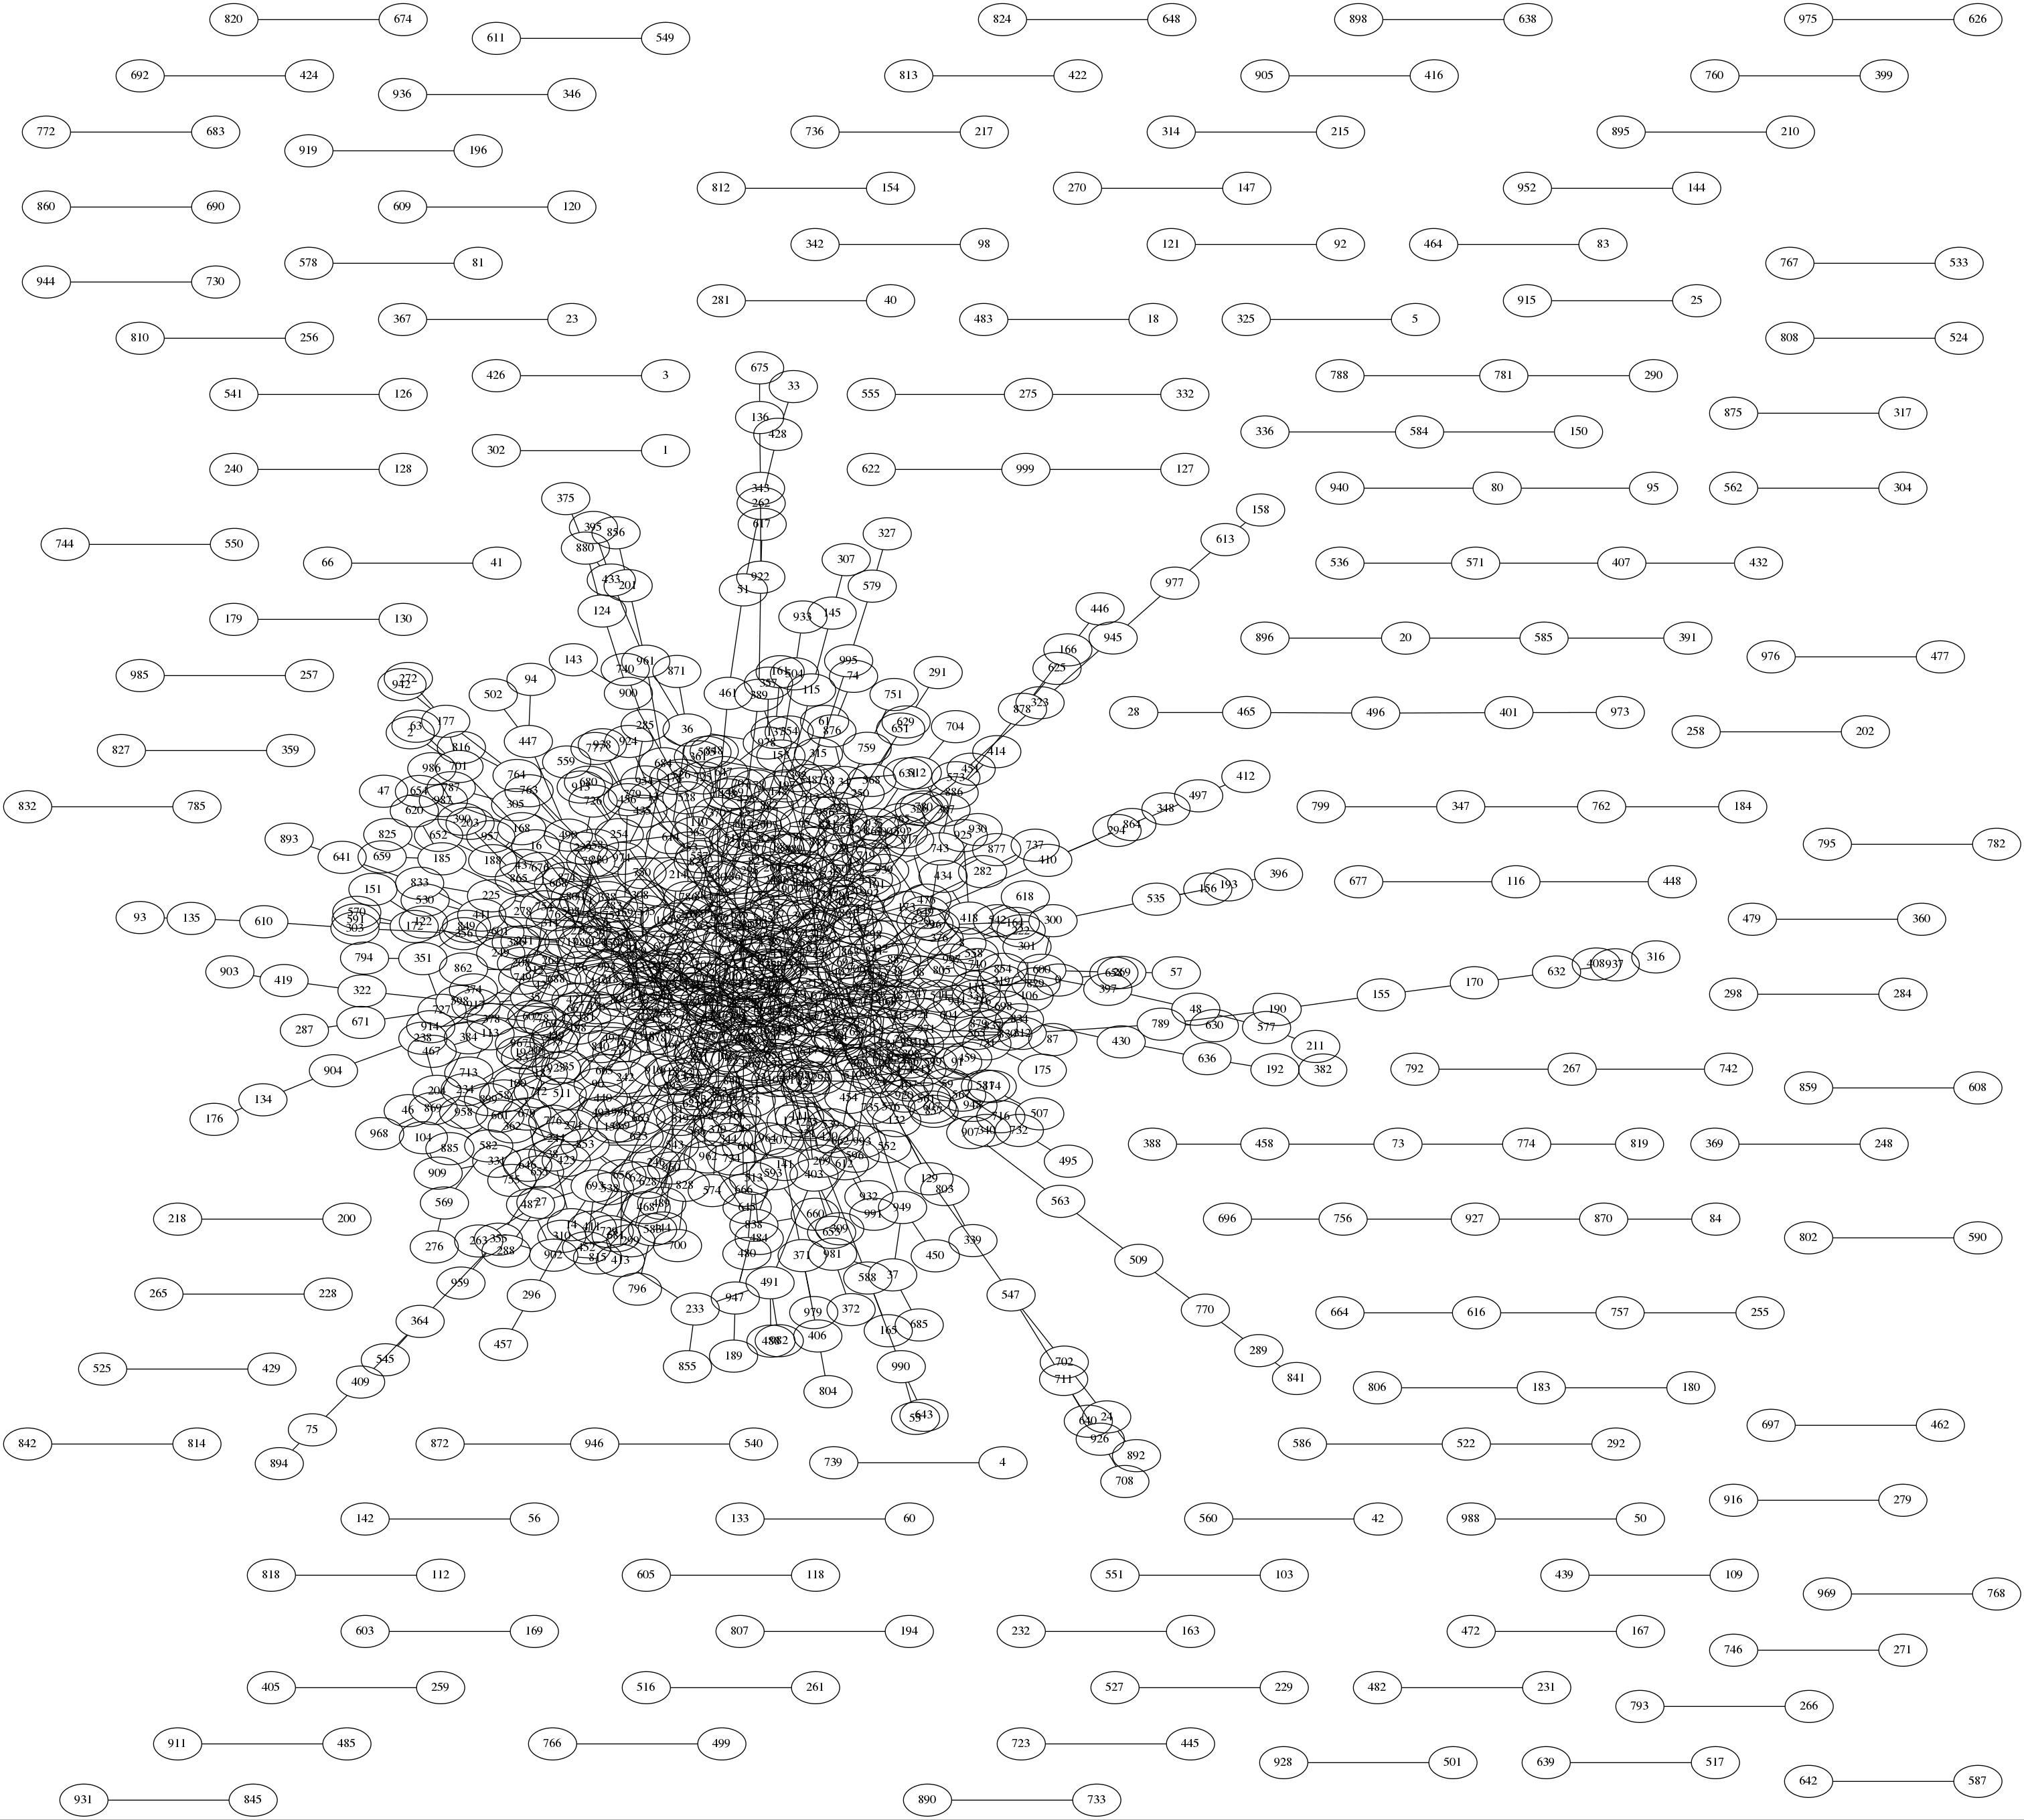
\includegraphics[width=\textwidth]{1000_5}
%       \caption{$|V|=1000$, $d=5$}
%   \end{sidewaysfigure}
% }